\documentclass[a4paper]{article} 
\addtolength{\hoffset}{-2.25cm}
\addtolength{\textwidth}{4.5cm}
\addtolength{\voffset}{-3.25cm}
\addtolength{\textheight}{5cm}
\setlength{\parskip}{0pt}
\setlength{\parindent}{0in}

%----------------------------------------------------------------------------------------
%	PACKAGES AND OTHER DOCUMENT CONFIGURATIONS
%----------------------------------------------------------------------------------------

\usepackage{blindtext} % Package to generate dummy text
\usepackage{charter} % Use the Charter font
\usepackage[utf8]{inputenc} % Use UTF-8 encoding
\usepackage{microtype} % Slightly tweak font spacing for aesthetics
\usepackage[english]{babel} % Language hyphenation and typographical rules
\usepackage{amsthm, amsmath, amssymb} % Mathematical typesetting
\usepackage{float} % Improved interface for floating objects
\usepackage[final, colorlinks = true, 
            linkcolor = black, 
            citecolor = black]{hyperref} % For hyperlinks in the PDF
\usepackage{graphicx, multicol} % Enhanced support for graphics
\usepackage{xcolor} % Driver-independent color extensions
\usepackage{marvosym, wasysym} % More symbols
\usepackage{rotating} % Rotation tools
\usepackage{censor} % Facilities for controlling restricted text
\usepackage{listings, style/lstlisting} % Environment for non-formatted code, !uses style file!
\usepackage{pseudocode} % Environment for specifying algorithms in a natural way
\usepackage{style/avm} % Environment for f-structures, !uses style file!
\usepackage{booktabs} % Enhances quality of tables
\usepackage{tikz-qtree} % Easy tree drawing tool
\tikzset{every tree node/.style={align=center,anchor=north},
         level distance=2cm} % Configuration for q-trees
\usepackage{style/btree} % Configuration for b-trees and b+-trees, !uses style file!
\usepackage{csquotes} % Context sensitive quotation facilities
\usepackage[yyyymmdd]{datetime} % Uses YEAR-MONTH-DAY format for dates
\renewcommand{\dateseparator}{-} % Sets dateseparator to '-'
\usepackage{fancyhdr} % Headers and footers
\pagestyle{fancy} % All pages have headers and footers
\fancyhead{}\renewcommand{\headrulewidth}{0pt} % Blank out the default header
\fancyfoot[L]{} % Custom footer text
\fancyfoot[C]{} % Custom footer text
\fancyfoot[R]{\thepage} % Custom footer text
\newcommand{\note}[1]{\marginpar{\scriptsize \textcolor{red}{#1}}} % Enables comments in red on margin

%----------------------------------------------------------------------------------------

\begin{document}

%-------------------------------
%	TITLE SECTION
%-------------------------------

\fancyhead[C]{}
\hrule \medskip % Upper rule
\begin{minipage}{0.295\textwidth} 
\raggedright
\footnotesize
Andrew Hayes \hfill\\   
21321503 \hfill\\
a.hayes18@nuigalway.ie
\end{minipage}
\begin{minipage}{0.4\textwidth} 
\centering 
\large 
CT255 Assignment 3\\ 
\normalsize 
Steganography\\ 
\end{minipage}
\begin{minipage}{0.295\textwidth} 
\raggedleft
\today\hfill\\
\end{minipage}
\medskip\hrule 
\bigskip

%-------------------------------
%	CONTENTS
%-------------------------------

\section{Problem 1}
\subsection{Code}
\begin{lstlisting}[language=Java]
import java.io.BufferedReader;
import java.io.BufferedWriter;
import java.io.FileReader;
import java.io.FileWriter;
import java.io.IOException;
import java.util.regex.Pattern;

public class Stegano1
{
    public static void main(String[] args) {
        // Strings to hold the arguments. mode is either A or E for "Add" or "Extract". 
        String mode, inputfile, outputfile, bitstring;  
        Boolean err = false;                                                    // Boolean to tell if the arguments were passed correctly or not 

        if (args.length > 1) {                                                  // checking that at least one argument was passed to main
            // assigning the mode & inputfile arguments
            mode = args[0];
            inputfile = args[1];
                
            if (inputfile.equals("")) {                                         // checking that an inputfile was provided (String was not empty)
                err = true;
            }
            else if ((mode.equals("A")) && (args.length > 3)){                  // checking if the mode is "Add" & that the number of arguments provided was greater than 3
                // assigning the outputfile & bitstring arguments
                outputfile = args[2];
                bitstring = args[3];
        
                if (outputfile.equals("") || bitstring.equals("")) {            // checking that neither the outputfile nor bitstring were empty strings
                    err = true;
                }
                else {
                    // hiding the bitstring
                    hide(inputfile, outputfile, bitstring);
                }
            }
            else if (mode.equals("E")){                                         // checking if the mode is "Extract"
                // retrieving (extracting) the bitstring from text   
                retrieve(inputfile);   
            }
            else {
                err = true;
            }
        }
        else {
            err = true;
        }
        
        if (err) {
            System.out.println();
            System.out.println("Use: Stegano1 <A:E><Input File><OutputFile><Bitstring>");
            System.out.println("Example to add a bitvector to a file: Stegano1 A inp.txt out.txt 0010101");
            System.out.println("Example to extract a bitvector from a file: Stegano1 E inp.txt");
            
        } 
    }
   
    // method to hide a bitstring in a copy the input file provided
    static void hide(String inpFile, String outFile, String bitString) {
        BufferedReader reader;                                                  // declaring a BufferedReader for the input file 
        BufferedWriter writer;                                                  // declaring a BufferedWriter for the output file
	
        try {
            // initialising the reader & writer to FileReaders of their respective files (inpFile & outFile)
            reader = new BufferedReader(new FileReader(inpFile));       
            writer = new BufferedWriter(new FileWriter(outFile));
            
            String line = reader.readLine();                                    // reading in the first line from the input file
            
            // will loop until there are no more lines to be read in from the input file (inpFile)
            while (line != null) {
               
                // if the bitString is not (yet) an empty String
                if (!bitString.equals("")) {

                    // if the first bit (char) of the bitString is 0
                    if (bitString.charAt(0) == '0') {                           // note: must use '' instead of "" for char literals
                        line = line.concat(" ");                                // concatenating a space to the end of the line (one space represents a 0)
                    }  
                    
                    // if the first bit of the bitString is 1
                    if (bitString.charAt(0) == '1') {
                        line = line.concat("  ");                               // concatenating two spaces to the end of the line (two spaces represents a 1)
                    }

                    // removing the first bit from the bitString now that it has been used
                    bitString = bitString.substring(1, bitString.length());     // replacing bitString with it's substring that goes from the second character to the last character
                }

                // writing the amended line to the output file
                writer.write(line);
                writer.newLine();

		        // reading the next line
		        line = reader.readLine();
            }

            // closing the reader & the writer
            reader.close();
            writer.close();
	    }

        // catching any IOExceptions
        catch (IOException e) {
	        e.printStackTrace();
	    }
    }
    
    // method to retrieve a hidden string from the input file provided
    static void retrieve(String inpFile) {
        BufferedReader reader;                                          // declaring a BufferedReader for the input file (inpFile)
        String message = "";

        try {
            reader = new BufferedReader(new FileReader(inpFile));       // initialising the reader to a FileReader of the input file (inpFile) 
            
            String line = reader.readLine();                            // reading in the first line from the input file
            
            // will loop until there are no more lines to be read in from the input file
            while (line != null) {

                // checking if the line ends in a space using a regular expression
                if (Pattern.matches(".* $", line)) {                    // (checking if the String line contains any amount of any characters, followed by a space followed by the end of a line)

                    // checking if the line ends in two spaces using a regular expression
                    if (Pattern.matches(".*  $", line)) {               // (checking if the String line contains any amount of any characters, followed by two spaces followed by the end of a line)
                        message = message.concat("1");                  // concatenating a "1" onto the message String (two spaces represent a "1")
                    }
                    else {                                              // essentially, this "else" means "if the line ends with one space but not two"
                        message = message.concat("0");                  // concatenating a "0" onto the message String (one space represents a "0")
                    }
                }
                else {                                                  // if the String does not end in a space, then there is no (more) message to read
                    break;
                }
                
                // reading the next line
	        	line = reader.readLine();
            }

            // closing in the reader
            reader.close();

            // checking if the message String is empty so that an error message can be printed if no hidden message was found
            if (message.equals("")) {
                message = "Error: No hidden message found!";
            }

            // printing out the message
            System.out.println(message);
	    } 
        // catching any IOExceptions
        catch (IOException e) {
	        e.printStackTrace();
	    }
    }
}
\end{lstlisting}

\subsection{Screenshot of Compilation \& Output}
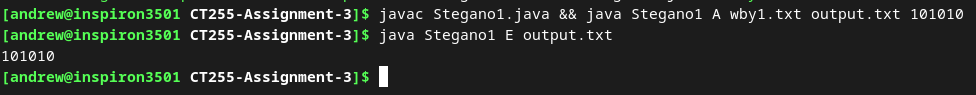
\includegraphics[width = 15cm]{output1.png}
\bigskip

%------------------------------------------------

\section{Problem 2}
\subsection{Code}
\begin{lstlisting}[language=java]
import java.io.BufferedReader;
import java.io.BufferedWriter;
import java.io.FileReader;
import java.io.FileWriter;
import java.io.IOException;
import java.util.regex.Pattern;

public class Stegano1
{
    public static void main(String[] args) {
        // Strings to hold the arguments. mode is either A or E for "Add" or "Extract". 
        String mode, inputfile, outputfile, bitstring;  
        Boolean err = false;                                                    // Boolean to tell if the arguments were passed correctly or not 

        if (args.length > 1) {                                                  // checking that at least one argument was passed to main
            // assigning the mode & inputfile arguments
            mode = args[0];
            inputfile = args[1];
                
            if (inputfile.equals("")) {                                         // checking that an inputfile was provided (String was not empty)
                err = true;
            }
            else if ((mode.equals("A")) && (args.length > 3)){                  // checking if the mode is "Add" & that the number of arguments provided was greater than 3
                // assigning the outputfile & bitstring arguments
                outputfile = args[2];
                bitstring = args[3];
        
                if (outputfile.equals("") || bitstring.equals("")) {            // checking that neither the outputfile nor bitstring were empty strings
                    err = true;
                }
                else {
                    // hiding the bitstring
                    hide(inputfile, outputfile, bitstring);
                }
            }
            else if (mode.equals("E")){                                         // checking if the mode is "Extract"
                // retrieving (extracting) the bitstring from text   
                retrieve(inputfile);   
            }
            else {
                err = true;
            }
        }
        else {
            err = true;
        }
        
        if (err) {
            System.out.println();
            System.out.println("Use: Stegano1 <A:E><Input File><OutputFile><Bitstring>");
            System.out.println("Example to add a bitvector to a file: Stegano1 A inp.txt out.txt 0010101");
            System.out.println("Example to extract a bitvector from a file: Stegano1 E inp.txt");
            
        } 
    }
   
    // method to hide a bitstring in a copy the input file provided
    static void hide(String inpFile, String outFile, String bitString) {
        // to encode 2 bits with just one symbol, i'm going to represent the binary digits as an analog represenation of the number it represents plus one
        // e.g., 00 will be represented as " " (1 space), 01 as "  " (2 spaces), 10 as "   " (3 spaces), and 11 as "    " (4 spaces)
        // the two bits are treated as a binary number, and then i add one to said binary number to get the number of spaces that will represent that number

        BufferedReader reader;                                                  // declaring a BufferedReader for the input file 
        BufferedWriter writer;                                                  // declaring a BufferedWriter for the output file
	
        try {
            // initialising the reader & writer to FileReaders of their respective files (inpFile & outFile)
            reader = new BufferedReader(new FileReader(inpFile));       
            writer = new BufferedWriter(new FileWriter(outFile));
            
            String line = reader.readLine();                                    // reading in the first line from the input file

            // checking if the number of bits in the bitstring is uneven, and if so, adding a '0' onto the end 
            if (bitString.length() % 2 != 0) { bitString = bitString.concat("0"); }
            
            // will loop until there are no more lines to be read in from the input file (inpFile)
            while (line != null) {
               
                // if the bitString is not (yet) an empty String
                if (!bitString.equals("")) {

                    // if the first 2-bit substring is 00, adding one space to the end of the line
                    if (bitString.substring(0,2).equals("00")) {
                        line = line.concat(" ");
                    }
                    // if the first 2-bit substring is 01, adding two spaces to the end of the line
                    else if (bitString.substring(0,2).equals("01")) {
                        line = line.concat("  ");
                    }
                    // if the first 2-bit substring is 10, adding three spaces to the end of the line
                    else if (bitString.substring(0,2).equals("10")) {
                        line = line.concat("   ");
                    }
                    // if the first 2-bit substring is 11, adding four spaces to the end of the line
                    else if (bitString.substring(0,2).equals("11")) {
                        line = line.concat("    ");
                    }
                    // removing the first two bits from the bitString now that they have been used
                    bitString = bitString.substring(2, bitString.length());     // replacing bitString with it's substring that goes from the third character to the last character
                }

                // writing the amended line to the output file
                writer.write(line);
                writer.newLine();

		        // reading the next line
		        line = reader.readLine();
            }

            // closing the reader & the writer
            reader.close();
            writer.close();
	    }

        // catching any IOExceptions
        catch (IOException e) {
	        e.printStackTrace();
	    }
    }
    
    // method to retrieve a hidden string from the input file provided
    static void retrieve(String inpFile) {
        BufferedReader reader;                                                  // declaring a BufferedReader for the input file (inpFile)
        String message = "";

        try {
            reader = new BufferedReader(new FileReader(inpFile));               // initialising the reader to a FileReader of the input file (inpFile) 
            
            String line = reader.readLine();                                    // reading in the first line from the input file
            
            // will loop until there are no more lines to be read in from the input file
            while (line != null) {
                // checking if the line ends in a space using a regular expression
                if (Pattern.matches(".* $", line)) {                            // (checking if the String line contains any amount of any characters, followed by a space followed by the end of a line)

                    if (Pattern.matches(".*    $", line)) {                     // checking if the line ends in four spaces using a regular expression
                        message = message.concat("11");                         // concatenating "11" onto the end of the message String (four spaces represents "11")
                    }
                    else if (Pattern.matches(".*   $", line)) {                 // checking if the line ends in three spaces using a regular expression
                        message = message.concat("10");                         // concatenating "10" onto the end of the message String (three spaces represents "10")
                    }
                    else if (Pattern.matches(".*  $", line)) {                  // (checking if the String line contains any amount of any characters, followed by two spaces followed by the end of a line)
                        message = message.concat("01");                         // concatenating a "1" onto the message String (two spaces represent a "1")
                    }
                    else {                                                      // essentially, this "else" means "if the line ends with one space but not two"
                        message = message.concat("00");                         // concatenating a "0" onto the message String (one space represents a "0")
                    }
                }
                else {                                                          // if the String does not end in a space, then there is no (more) message to read
                    break;
                }
                
                // reading the next line
	        	line = reader.readLine();
            }

            // closing in the reader
            reader.close();

            // checking if the message String is empty so that an error message can be printed if no hidden message was found
            if (message.equals("")) {
                message = "Error: No hidden message found!";
            }

            // printing out the message
            System.out.println(message);
	    } 
        // catching any IOExceptions
        catch (IOException e) {
	        e.printStackTrace();
	    }
    }
}
\end{lstlisting}
\subsection{Output}
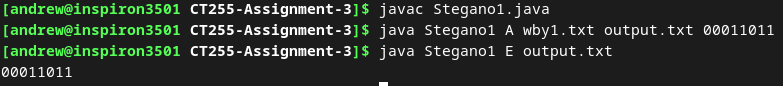
\includegraphics[width = 15cm]{output2.png}

\end{document}
